\begin{figure}
  \centering

  \begin{subfigure}{\linewidth}
    
\includegraphics[width=\linewidth]{Figures/steps-a.pdf}
    \caption{\textbf{Early-stage training.}
    After only one to two thousand training steps, the HY1.5-based bidirectional model has not yet acquired effective camera controllability.}
  \end{subfigure}

  \vspace{0.5em}

  \begin{subfigure}{\linewidth}
    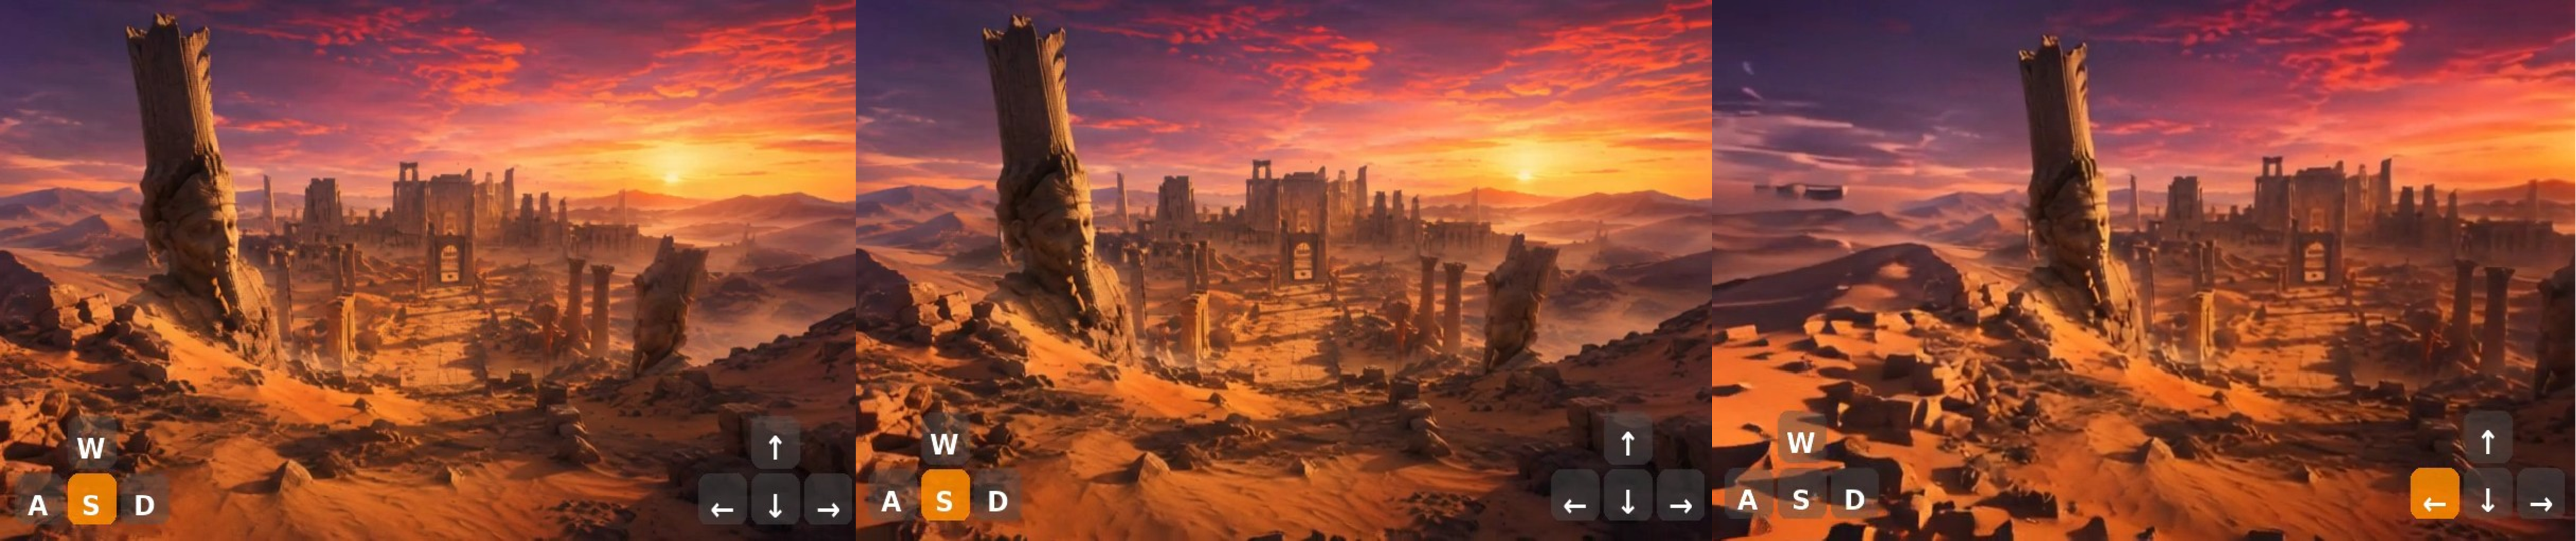
\includegraphics[width=\linewidth]{Figures/steps-b.pdf}
    \caption{\textbf{Emerging controllability.}
    After around five thousand training steps, the model begins to respond to camera-control signals, but the controllability is still unstable.}
  \end{subfigure}

  \vspace{0.5em}

  \begin{subfigure}{\linewidth}
    
\includegraphics[width=\linewidth]{Figures/steps-c.pdf}
    \caption{\textbf{Strong controllability.}
    After eight thousand training steps, the model achieves substantially stronger and more reliable camera-controllable generation.}
  \end{subfigure}

  \caption{\textbf{Effect of training steps on camera-controllable generation.}
  Using HY1.5 as an example, we observe that camera controllability emerges progressively during training: the model is largely uncontrollable at one to two thousand steps, starts to acquire controllability around five thousand steps, and reaches strong controllability after eight thousand steps.}
  \label{fig:ablation-steps}

\end{figure}